%************************************************************************
\section{System Models}
%************************************************************************

This section describes our system model that we adopt for our empirical analysis. We will be using a dynamical system, together with simplified versions of that system.

\subsection{Model Overview}

In this paper, we use the three-tank system shown in Fig.~\ref{fig:three_tanks} as tour system model. The three tanks are denoted as $T_1$, $T_2$, and $T_3$. They all have the same area $A_1 = A_2 = A_3.$
% = 3~[\textrm{m}^2]$. %The experiments are performed assuming the gravity $g = 10$ and the liquid with density $\rho = 1$.

\begin{figure}[htb]
  \centering
%  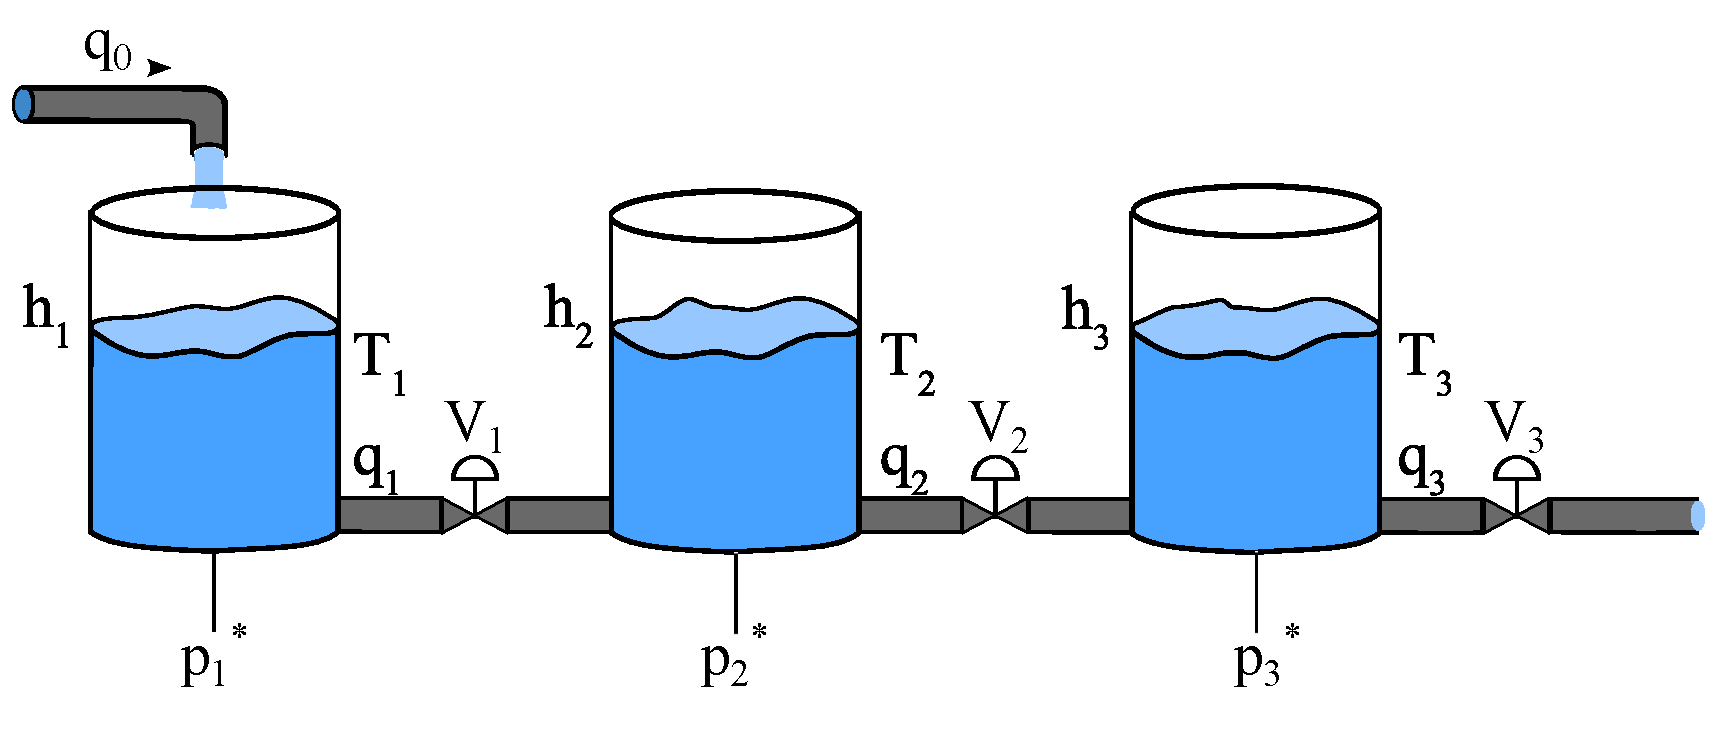
\includegraphics[width=\columnwidth]{3-tanks.pdf}
  \caption{Diagram of the three-tank system.}
  \label{fig:three_tanks}
\end{figure}
\par\noindent

Tank $T_1$ gets filled from a pipe, with measured flow $q_0$. Hence, $\vec{u}=\{q_0\}$% with a constant flow of $1.5~[\textrm{m}^3/\textrm{s}]$. 

$T_1$ drains into $T_2$ via a pipe $q_1$. The liquid level is denoted as $h_1$. There is a pressure sensor $p_i$ connected to $T_i$, for $i=1,2,3$.
In Eq.~\ref{eq:ode1}, the coefficient $\kappa_1$ is used to model the area of the drainage hole and its friction factor through a physical valve $\kappa_1$.% We emphasize the use of $k_1$ because, later, we will be ``diagnosing'' our system in term of changes in $k_1$. Consider a physical valve $R_1$ between $T_1$ and $T_2$ that constraints the flow between the two tanks. We can say that the valve changes proportionally the cross-sectional drainage area of $q_1$ and hence $k_1$. 
The diagnostic task will be to compute the true value of $\kappa_1$, given $p_1$.

%================================================================
\subsection{Non-Linear Model}
%\begin{eqnarray}
%\label{eq:h_1}
%\frac{d h_1}{dt} = \frac{q_0 - \kappa_1 \sqrt{h_1 - h_2}}{A_1}\label{eq:ode1}
%\end{eqnarray}

\begin{eqnarray}
\frac{d h_1}{dt} & = & \frac{1}{A_1}\left[  - \kappa_1 \sqrt{h_1 - h_2} + q_0 \right],    \label{eq:ode1} \\
\frac{d h_2}{dt} &  = & \frac{1}{A_2}\left[   \kappa_{1} \sqrt{h_{1}-h_{2}} - \kappa_2 \sqrt{h_2-h_3}\right],\\
\frac{d h_3}{dt} & = & \frac{1}{A_3}\left[   \kappa_{2} \sqrt{h_2-h_3} - \kappa_3 \sqrt{h_3}\right].
\end{eqnarray}


Finally, the pressure at the bottom of each tank is obtained from the height:
\begin{eqnarray}\label{eq:pressure}
p_i = g\,h_i  
\end{eqnarray}
where $i$ is the tank index ($i \in \{1, 2, 3\}$).

When we make the following definitions:
\begin{equation}
\vec{x}(t) = \left[ \begin{array}{c}
h_1 \\ h_2 \\ h_3 \end{array}
\right],
%%%%%%%%%%%%%%%%%%%%%%%%%%%%%%%%%
~~ \vec{u}(t)  = \left[ \begin{array}{c}
q_0 \\ 0 \\ 0 \end{array}
\right],
%%%%%%%%%%%%%%%%%%%%%%%%%%%%%%%%%
~~ \vec{\omega}(t) = \left[ \begin{array}{c}
\omega_1 \\ \omega_2 \\ \omega_3 \end{array}
\right],
\end{equation}
we can rewrite the (fault-free) model in state-space form
\begin{equation}\label{state-space}
\frac{d \vec{x}(t)}{dt} = \psi (\vec{x}(t)) + \vec{u}(t)) 
%+ \varsigma(\vec{\omega}(t))
\end{equation}




\subsection{Qualitative Model}
%************************************************************************

For the qualitative model we replace the non-linear sub-function
$ \sqrt{h_i - h_j}$ with the qualitative sub-function $M^+(h_i - h_j)$,
where $M^+$ is the set of reasonable functions $f$ such that $f' > 0$ on the interior of its domain \citep{kuipers1994composition}.

\begin{eqnarray}
\frac{d h_1}{dt} & = & \frac{1}{A_1}\left[  - \kappa_1  M^+(h_1 - h_2) + q_0 \right]    \label{eq:qual-ode1} \\
\frac{d h_2}{dt} &  = & \frac{1}{A_2}\left[   \kappa_{1} M^+(h_{1}-h_{2}) - \kappa_2 M^+(h_2-h_3)\right],\\
\frac{d h_3}{dt} & = & \frac{1}{A_3}\left[   \kappa_{2} M^+(h_2-h_3) - \kappa_3 M^+(h_3)\right].
\end{eqnarray}

The tank-heights are constrained to be non-negative. As a consequence,
we can discretize the $h_i$ to take on values $\{+, 0\}$, which means that $M^+(h_i - h_j)$ can take on values $\{+, 0, -\}$. 
The domain for $\frac{d h_1}{dt}$ must be $\{+, 0, -\}$, since $q_0$ is non-negative and each  $M^+(h_i - h_j)$ can take on values $\{+, 0, -\}$.
With this, we obtain the simplified (fault-free) equations:
\begin{eqnarray}
\frac{d h_1}{dt} & = &   -  M^+(h_1 - h_2) + q_0,  \label{eq:qual-ode-simple} \\
\frac{d h_2}{dt} &  = &    M^+(h_{1}-h_{2}) - M^+(h_2-h_3),\\
\frac{d h_3}{dt} & = &    M^+(h_2-h_3) - M^+(h_3).
\end{eqnarray}


\subsection{Linear Model}
%************************************************************************

The general form for a linear version of  equation \ref{state-space} is
\begin{equation}\label{linear-state-space}
\frac{d \vec{x}(t)}{dt} = \mathbf{A} \vec{x}(t) + \mathbf{B} \vec{u}(t)) + \mathbf{C} \vec{\omega}(t),
\end{equation}
where $\mathbf{A}, \mathbf{B}$ and $\mathbf{C}$ are linear matrices.

For the linear 3-tank model we replace the non-linear sub-function
$ \sqrt{h_i - h_j}$ with the linear sub-function $\gamma_{ij} (h_i - h_j)$, where $\gamma_{ij}$ is a parameter (to be estimated) governing the flow between tanks $i$ and $j$. We obtain the following system equations:

\begin{eqnarray} \label{eq:linear-ode1}
\frac{d h_1}{dt} & = & \frac{1}{A_1}\left[  - \kappa_1 \gamma_{12} (h_1 - h_2) + q_0 \right]  \\%  \label{eq:linear-ode1} \\
\frac{d h_2}{dt} &  = & \frac{1}{A_2}\left[   \kappa_{1} \gamma_{12} (h_{1}-h_{2}) - \kappa_2 \gamma_{23} (h_2-h_3)\right],\\
\frac{d h_3}{dt} & = & \frac{1}{A_3}\left[   \kappa_{2} \gamma_{23} (h_2-h_3) - \kappa_3 \gamma_{3} h_3\right].
\end{eqnarray}

%If we set $\lambda_{ij}= \frac{\kappa_i}{A_j} \gamma_{ij}$, then we obtain
%%%ORIGINAL VERSION
%\begin{equation}  \label{eq:linear-matrix}
%\frac{d {\vec h}}{dt}  =  
%\left[ \begin{array}{ccc}
%-T_{11}\gamma_{12} &  T_{11}\gamma_{12} & 0 \\
%-T_{12}\gamma_{12} & -( T_{12}\gamma_{12} +  T_{22}\gamma_{23}) & T_{22}\gamma_{23} \\
%0 &  T_{22}\gamma_{23} & -(  T_{22}\gamma_{23} + T_{33}\gamma_{3}) \\  
%\end{array} \right]
%%-------------------
%\left[ \begin{array}{c} h_1 \\ h_2 \\ h_3 \end{array} \right]
%%%%%%%%%%%%%%%
%+  \left[ \begin{array}{c} q_0 \\ 0 \\ 0 \end{array} \right]
%\end{equation}

If we set $\lambda_{ij}= \frac{\kappa_i}{A_j}$, then we obtain the fault-free representation
\begin{equation}  \label{eq:linear-matrix}
\frac{d {\vec h}(t)}{dt}  =  
\mathbf{A}
%-------------------
\left[ \begin{array}{c} h_1 \\ h_2 \\ h_3 \end{array} \right]
%%%%%%%%%%%%%%
+  \left[ \begin{array}{c} q_0 \\ 0 \\ 0 \end{array} \right]
\end{equation}

where
\begin{equation}  \label{eq:A-matrix}
\mathbf{A}  =  
\left[ \begin{array}{ccc}
-\lambda_{11}\gamma_{12} &  \lambda_{11}\gamma_{12} & 0 \\
-\lambda_{12}\gamma_{12} & -( \lambda_{12}\gamma_{12} +  \lambda_{22}\gamma_{23}) & \lambda_{22}\gamma_{23} \\
0 &  \lambda_{22}\gamma_{23} & -(  \lambda_{22}\gamma_{23} + \lambda_{33}\gamma_{3}) \\  
\end{array} \right]
%-------------------
\end{equation}

%=======================================
\subsection{Fault Models}
%=======================================
This section describes the fault models we specify. We adopt two classes of model, \textit{weak} and \textit{strong}.
A \textit{weak model} specifies nominal behaviour only, so that a fault corresponds to any behavious deviating from nominal.
A \textit{strong model} specifies the dynamics of the fault.
